%%%%%%%%%%%%%%%%%%%%%%%%%%%%%%%%%%%%%%%%%%%%%%%%%%%%%%%%%%%%%%%%%%% 
%                                                                 %
%                            CHAPTER ONE                          %
%                                                                 %
%%%%%%%%%%%%%%%%%%%%%%%%%%%%%%%%%%%%%%%%%%%%%%%%%%%%%%%%%%%%%%%%%%%
\chapter{Introduction}
\section{Motivation}
Phyllosilicate clay minerals such as montmorillonite have been of interest to researchers of various domains for more than fifty years. Many different aspects of this material have been studied, ranging from its hydration and swelling properties \cite{aldrich1944hydration}, to its chemical properties, such as catalyzing the formation of RNA oligomers \cite{joshi2009mechanism}. Being a safe, naturally occurring material, it has found a wide variety of uses such as in pharmaceuticals, cosmetics, and oil refining \cite{hartwell1965diverse}.

Having found such a plethora of uses, its maintained interest over the years is understandable. As previously mentioned, a main industrial use for the material is its use as a catalyst for chemical reactions \cite{hartwell1965diverse}. More recently however, these known catalytic properties have expanded to include the catalyzation of RNA oligomers as expanded by Prakash Joshi, Michael Aldersley, John Delano, and James Ferris here at Rensselaer Polytechnic Institute (RPI) \cite{joshi2009mechanism}, \cite{aldersley2011role}. In addition to this fact, montmorillonite has also been shown to help catalyze the formation of vesicles from fatty acid micelles as shown by Hanczyc, Fujikawa, and Szostak \cite{hanczyc2003experimental}. The combination of these two catalytic capabilities has increased the interest of montmorillonite amongst biochemists and has incorporated montmorillonite into some theories of abiogenisis, as a possible candidate for having been the catalyst for the first protocells, and precursors of life on Earth \cite{hanczyc2003experimental}.

The conditions allowing montmorillonites to maximize their catalytic properties in terms of RNA oligomer formation has been previously researched \cite{aldersley2011role}, \cite{aldersley2011evaluation}, but much is still unknown about the exact physics and chemistry governing these processes. Its importance in industrial applications, as well as to the theory of abiogenisis in conjunction with this lack of basic understanding behind the underlying principles is what has prompted this research.

\section{Background and Previous Works}
\subsection{Structure of Montmorillonite}
Montmorillonite is the most prominent form of smectite, which is in turn a type of phyllosilicate. The most basic structure of montmorillonite is a sheet formed by two tetrahedral sheets which sandwich a dioctahedral sheet \cite{sposito1984surface}. Such a structure is referred to as a 2:1 structure, in reference to being composed of two tetrahedral sheets and one dioctahedral sheet. The tetrahedral sheets are in general composed of silica, with aluminum substitutions, and the dioctahedral sheet is alumina which may also be substituted by iron and magnesium. In all, the chemical formula for montmorillonite is given as
\begin{equation*}
	[(Si_{3.88}Al_{0.12})^{IV}(Al_{1.64}Fe_{0.05}^3Mg_{0.36})^{VI}O_{10}(OH)_2]_2
\end{equation*}
where the superscripts $IV$ and $VI$ refer to the coordination of the tetrahedral and dioctahedral structures respectively \cite{van1977introduction}. A diagram of these structures is presented in Figure ~\ref{fig:clay_structure}.
\resetfootnote
\begin{figure}
	\centering
	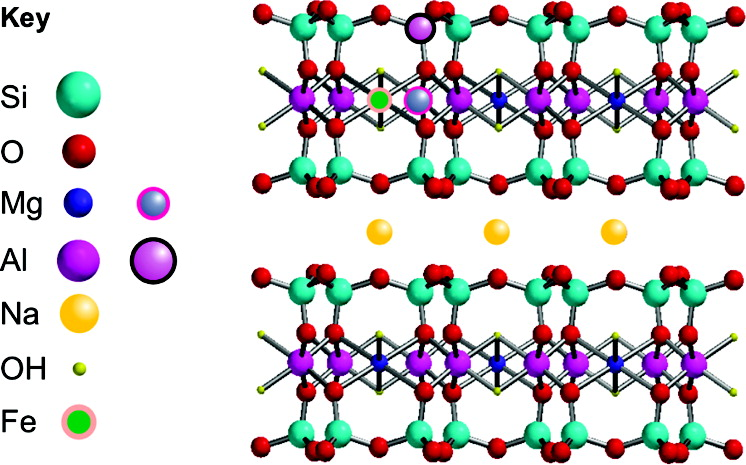
\includegraphics[scale=1.75]{images/clay_structure.jpg}
	\caption{Diagram of montmorillonite unit cell\protect\footnotemark. Outlined atoms indicate substitutions \cite{joshi2009mechanism}.}
	\label{fig:clay_structure}
\end{figure}
\footnotetext{ Reprinted with permission from P.C. Joshi, M.F. Aldersley, J.W. Delano, and J.P. Ferris, “Mechanism of montmorillonite catalysis in the formation of RNA oligomers,” \textit{J. Amer. Chem. Soc.}, vol. 131, no. 37, pp. 13 369–13 374, Sept. 2009. Copyright 2009 American Chemical Society.}

The substitutions in the clay cause a buildup of a net negative charge on the surfaces of the clay structure due to the provided supplemental electrons. The magnitude of this charge depends on the number and type of substitutions. Due to these variations, different types or varieties of montmorillonite are known to have different surface charges. This value can range from 0.66 to 0.98 per O$_{20}$(OH)$_4$ formula unit \cite{joshi2009mechanism}, \cite{newman1987chemical}. As the Coulomb force between sheets of clay would naturally repel them, positively charged exchangeable interlaminar cations are present between the sheets, leading to a net neutral charge and neutralizing the repulsive force between sheets \cite{mering1953role}. Typically, these cations are alkali or alkaline earth metals such as Na, Li, K, Mg, or Ca \cite{berend1995mechanism}. For the work conducted within this thesis, only montmorillonite samples with interlaminar cations of Li, Na, and K were used.

\subsection{Swelling Properties}
In a completely dry sample of montmorillonite, the interlaminar cations are located in the hexagonal cavities on the external surfaces of each individual clay sheet. For Na montmorillonite, this results in a basal spacing between sheets of approximately $d_{001}=9.6\angstrom$ \cite{cases1992mechanism}. This spacing for dry montmorillonites is dependent on the valence or radius of the exchangeable cation of the particular sample in question \cite{mering1953role}. While both Li and Na montmorillonites have a basal spacing of approximately 9.6$\angstrom$, it is found that this value increases to 9.95$\angstrom$ for K, 10.25 - 10.6$\angstrom$ for Rb, and 10.7 - 11.5$\angstrom$ montmorillonites \cite{berend1995mechanism}.

Water in the vicinity of montmorillonite has the tendency to be absorbed by the mineral. These water molecules may accumulate on the surfaces of the clay structure, but are also intercalated between the clay sheets, solvating the exchangeable cations \cite{aldrich1944hydration}, \cite{mering1946hydration}. During this process, the cations will be unseated from the hexagonal cavities, and be more freely accessed by the intercalated water \cite{mering1953role}. Upon sufficient water content, usually provided in the form of water vapor from the ambient atmosphere, a monolayer of water will form between the clay sheets. Increasing the availability of water (by increasing the relative humidity in most cases) will eventually facilitate the formation of a bilayer of water, and subsequently a trilayer and so on. With each added layer of water, the basal spacing between sheets also increases. The type of exchangeable cation which is present in the clay will dictate these spacings, as well as how many layers of water may form \cite{mering1964gonflement}.

Often, it is possible to achieve up to three layers of water between sheets for Li, and Na montmorillonite. For K montmorillonite however, it is difficult to obtain a bilayer and for cations with a valence larger than this, such as the cases with Cs and Rb, only a monolayer is possible \cite{mering1964gonflement}. Spacings for a monolayer of water are usually in the vicinity of $d_{001}=12.0\angstrom$ for Li, and $d_{001}=12.5\angstrom$ for Na, K, Rb, and Cs exchanged montmorillonites. A bilayer hydrate is represented by a basal spacing of $d_{001}=15.5$ - $16.0\angstrom$ \cite{berend1995mechanism}. Trilayers typically present with $d_{001}\approx 18.1\angstrom$ \cite{cases1992mechanism}. The relative humidity required to obtain a certain number of water layers between clay sheets is highly dependent on the exchangeable cation. For example, it has been shown that a sample of Na montmorillonite kept at a relative humidity of $p/p_0=0.98$, has a basal spacing of $d_{001}=15.76\angstrom$. Similarly prepared K montmorillonite kept at a humidity of $p/p_0=0.97$ for more than four times as long as the Na sample was found to have a basal spacing of only $d_{001}=12.08\angstrom$ \cite{berend1995mechanism}. Jacques Méring and Rachel Glaeser were also able to show that it is easier to hydrate a montmorillonite which has exchangeable cations of a higher valence (such as Ca$^{2+}$), as the non-local charge cancellation increases the energy of the system, making it easier to solvate these cations \cite{mering1953role}.

A final aspect of the swelling properties of montmorillonite, which must be mentioned, is the fact that the process is very heterogeneous. By stating this, it is meant that a monolayer of water does not form homogeneously and instantly in the clay. What instead will happen is more of the interlaminar surface will be covered with a monolayer of water as the relative humidity increases, until there is a complete and homogeneous monolayer. At this point, a bilayer will begin to form as the humidity is continually increased. This process was thoroughly investigated by Cases et al. in their 1992 Langmuir paper \cite{cases1992mechanism}.

\subsection{Vibrational Modes of Intercalated Water}
Infrared spectroscopy has long been used to investigate the vibrational modes within the water molecule. For many years this methodology has been applied to investigate the specific behavior of the water which is intercalated in montmorillonite \cite{madejova2003ftir}. There are three principal vibrational modes of interest for water: symmetric O-H stretching ($\nu_1$), H-O-H bending or deformation ($\nu_2$), and asymmetric O-H stretching ($\nu_3$). One may find a depiction of these three modes in Figure~\ref{fig:water_vibrations}. It must be noted that these are all vibrations of the covalent bonds within a water molecule, and not vibrations which may occur in the hydrogen bond which forms between a hydrogen atom of one water molecule and the oxygen atom of another.

\begin{figure}
	\centering
	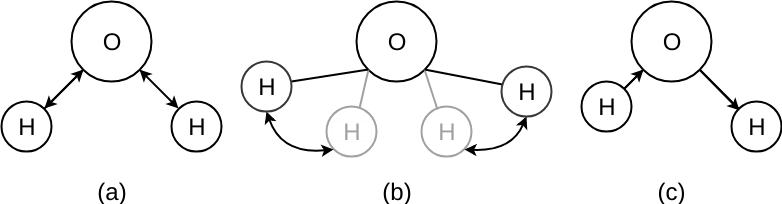
\includegraphics[scale=0.55]{images/water_vibrations.png}
	\caption{Vibrational modes of water: (a) depicts the symmetric stretching mode, (b) the bending or deformation mode, and (c) the asymmetric stretching mode.}
	\label{fig:water_vibrations}
\end{figure}

For liquid water, these modes are usually assigned frequencies of $\nu_1=3280cm^{-1}$, $\nu_2=1645cm^{-1}$, and $\nu_3=3490cm^{-1}$ \cite{eisenberg2005structure}. In liquid water, there is also an overtone of $\nu_1+\nu_2+\nu_3$ located at $3404cm^{-1}$ \cite{max2009isotope}. Although the intercalated water is in a liquid state, the frequencies of these modes are not the same as those of bulk water. The values of these frequencies for water intercalated in montmorillonite has been very well cataloged by Jana Madejová and Peter Komadel in their 2001 paper. In analyzing the infrared spectra of montmorillonite samples, they have assigned the water deformation mode to $\nu_2\approx 1632cm^{-1}$ and the stretching mode to $\nu_1\approx 3393cm^{-1}$ \cite{madejova2001baseline}. Their exact reported values vary slightly depending on location where the montmorillonite sample was taken from. A more in depth explanation of the location of these modes and the effects of exchangeable cation and hydration shall be given in chapter 3.

\section{Overview of this Work}
This thesis builds upon the already extensive body of knowledge on the subject, looking at some old problems from a new point of view, while also examining a new theory. Firstly, the hydration properties of montmorillonite were once again examined. Using X-ray Diffraction (XRD), the hydration of pressed disks of montmorillonite was examined. After being left in a desiccator at controlled humidity levels, the number of layers of water intercalated between clay sheets was measured for each disk by examining the distance between clay sheets. The goal of this experiment was to determine a simple but also effective method to accurately control the hydration of the clay samples, leaving either no water, a monolayer, bilayer, or trilayer of water between clay sheets, depending on the interlaminar cation which is present. One may find this portion of the thesis treated in chapter 2.

A novel, previously unexplored hypothesis is at the center of the second aspect of this work. The catalytic properties of montmorillonite previously discussed, have been shown to have a dependence on the pH of the clay used \cite{joshi2009mechanism}. To further explore this trend, infrared spectra of montmorillonite samples of varying interlaminar cation and pH values ranging from 3 to 10, were collected and analyzed. From the spectra of montmorillonite, one is able to observe the frequencies, and therefore corresponding energies of the O-H stretching mode, and the H-O-H deformation or "scissoring" mode of the water molecules which are intercalated. The energies of these modes were analyzed as a function of the pH of the clay, interlaminar cation, and origin of the clay sample. While infrared spectroscopy has been previously used to characterize clay minerals, no known work has been found examining pH dependencies. Due to the impact this could play on montmorillonite's ability to act as a catalyst, these results could play an important role in the fields of biochemistry and life sciences, as well as to Corning with their Life Sciences product line of laboratory glassware. This part of the research is outlined in chapter 3.

Finally, an attempt to model these montmorillonite-water surface interactions using molecular dynamics (MD) simulations was made. In this portion, two different modeling methods were attempted: one using Reax Force Fields which allow for the simulation of chemical reactions in MD simulations, and a more traditional MD approach, using standard Leonard-Jones and Coulomb potentials. Different approximations for the water molecules were also made for each of these options, where respectively the molecules were allowed to dissociate, and a flexible water model, where the O-H bonds and the angle between the two hydrogen atoms were both treated with harmonic potentials. Details pertaining to these simulations are given in chapter 4.

Also presented are considerations for future work on this subject, and future steps which are currently being considered to further examine this system, and better describe the interactions between intercalated molecules themselves, as well as with the clay surface.
 

%%% Local Variables: 
%%% mode: latex
%%% TeX-master: t
%%% End: 
